\section{Resultados}
\label{sec:resultados}

Nesta seção, são apresentados os resultados obtidos na avaliação dos modelos de classificação aplicados ao índice multivariado de poluição do ar. A análise contempla tanto o desempenho global dos classificadores quanto sua performance específica por classe, permitindo uma avaliação comparativa detalhada das abordagens consideradas.

A Tabela~\ref{tab:performance_nivel} apresenta os valores de acurácia e F1-score por classe do índice de poluição no conjunto de teste. Observa-se, de forma consistente entre os modelos avaliados, melhor desempenho na classe \textit{Moderado}, a qual concentra a maior parcela das observações e apresenta padrões mais estáveis no espaço de atributos.

Nas classes extremas (\textit{Muito baixo} e \textit{Crítico}), os valores das métricas exibem maior variabilidade entre os modelos. Esse comportamento indica maior dificuldade de separação nessas regiões do índice, que correspondem aos quantis inferiores e superiores da distribuição e estão mais sujeitas a sobreposição no espaço das variáveis preditoras.

Entre os modelos avaliados, as abordagens não lineares, em especial o MLP, apresentam valores de F1-score superiores nas classes críticas, indicando melhor equilíbrio entre precisão e revocação. Esse resultado sugere maior capacidade desses modelos em capturar relações não lineares entre as variáveis de entrada e as classes do índice. Ainda assim, modelos lineares, como Regressão Logística e LDA, mantêm desempenho competitivo, sobretudo nas classes intermediárias.
\begin{table}[ht]
\centering
\caption{Desempenho dos modelos por classe do índice de poluição.}
\label{tab:performance_nivel}
\begin{tabular}{l l c c c c c}
\toprule
Classe & Métrica & Logistic Reg. & LDA & KNN & MLP & QDA \\
\midrule
Muito baixo & Acc & \textbf{0.809} & 0.689 & 0.799 & \textbf{0.809} & 0.804 \\
Muito baixo & F1  & \textbf{0.841} & 0.729 & 0.811 & 0.831 & 0.834 \\
\midrule
Baixo & Acc & 0.789 & 0.784 & 0.764 & 0.767 & \textbf{0.817} \\
Baixo & F1  & 0.776 & 0.749 & 0.758 & 0.764 & \textbf{0.781} \\
\midrule
Moderado & Acc & 0.876 & 0.855 & \textbf{0.884} & 0.878 & 0.839 \\
Moderado & F1  & 0.858 & 0.854 & 0.861 & \textbf{0.862} & 0.846 \\
\midrule
Alto & Acc & 0.775 & \textbf{0.813} & 0.758 & 0.808 & 0.794 \\
Alto & F1  & 0.786 & 0.796 & 0.782 & \textbf{0.811} & 0.777 \\
\midrule
Crítico & Acc & 0.803 & 0.779 & 0.798 & \textbf{0.832} & 0.779 \\
Crítico & F1  & 0.846 & 0.850 & 0.836 & \textbf{0.872} & 0.837 \\
\bottomrule
\end{tabular}
\end{table}


A Figura~\ref{fig:mlp_confusion_matrix} apresenta a matriz de confusão do modelo MLP no conjunto de teste. Observa-se que a maioria dos erros de classificação ocorre entre classes adjacentes do índice de poluição, comportamento coerente com a natureza ordinal das classes definidas.

Não se verificam confusões relevantes entre classes extremas, o que indica que o modelo preserva a ordenação semântica implícita no problema de classificação.

\begin{figure}[h]
\centering
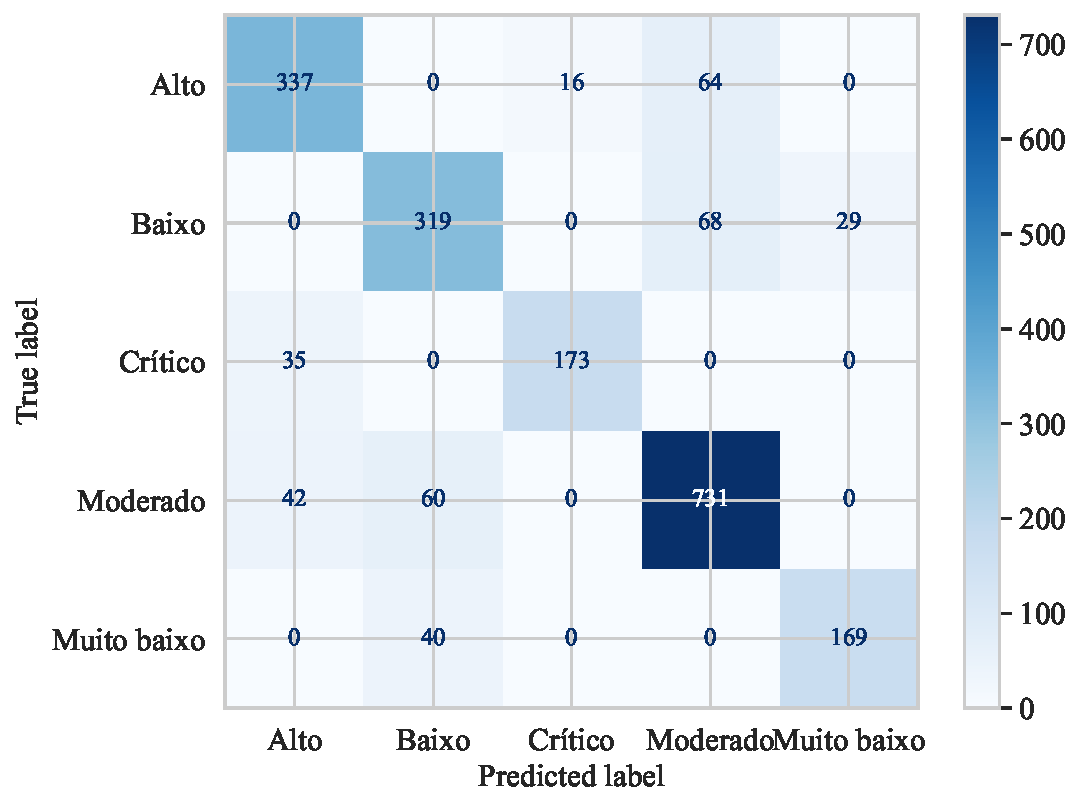
\includegraphics[width=\columnwidth]{figures/mlp_confusion_matrix.pdf}
\caption{Matriz de confusão do modelo MLP no conjunto de teste.}
\label{fig:mlp_confusion_matrix}
\end{figure}

A Tabela~\ref{tab:desempenho_modelos} resume o desempenho global dos modelos considerando a acurácia total e o F1-score macro. O MLP apresentou o melhor desempenho agregado, seguido de perto pela Regressão Logística.

Esses resultados indicam que, embora modelos não lineares apresentem vantagem marginal em desempenho global, abordagens lineares bem ajustadas permanecem competitivas no contexto do índice multivariado proposto.

\begin{table}[H]
\centering
\caption{Desempenho global dos modelos no conjunto de teste.}
\label{tab:desempenho_modelos}
\begin{tabular}{l c c}
\toprule
Modelo & Accuracy & F1\_macro \\
\midrule
MLP                 & \textbf{0.8301} & \textbf{0.8278} \\
Logistic Regression & 0.8243 & 0.8213 \\
QDA                 & 0.8161 & 0.8149 \\
KNN                 & 0.8176 & 0.8096 \\
LDA                 & 0.8080 & 0.7956 \\
\bottomrule
\end{tabular}
\end{table}
